\documentclass[12pt, a4paper]{article}
\usepackage[margin=1in]{geometry}
\usepackage{graphicx}
\usepackage{natbib}
\usepackage{hyperref}
\usepackage[utf8]{inputenc}
\usepackage{CJKutf8}

\title{Shinto Rituals and the Spiritual Significance of the Catastrophe in Japan}
\author{Hiroshi Fujita\thanks{Department of Religious Studies, University of Tokyo, Tokyo, Japan. Email: hfujita@u-tokyo.ac.jp} \and Yumi Miyamoto\thanks{Department of Anthropology, Kyoto University, Kyoto, Japan. Email: ymiyamoto@kyoto-u.ac.jp}}
\date{May 2026}

\begin{document}

\maketitle

\begin{abstract}
This study explores the role of Shinto rituals and beliefs in shaping Japanese responses to the catastrophic events of 2025, including the emergence of portals and dungeons. Through a combination of participant observation and interviews with Shinto priests and practitioners, the authors investigate how these events have been interpreted within the Shinto worldview and how they have influenced ritual practices and spiritual discourses. The findings suggest that the catastrophe has been seen as a manifestation of the power of the kami (gods and spirits) and as a call for humans to restore harmony with the natural and supernatural worlds. The paper discusses the ways in which Shinto rituals, such as purification ceremonies and offerings, have been adapted to address the spiritual challenges posed by the portals and dungeons, and how they have provided a source of comfort and resilience for many Japanese people in the face of the post-catastrophe reality.
\end{abstract}

\section{Introduction}
The emergence of mysterious portals and dungeons across Japan in 2025 has had a profound impact on the nation's spiritual landscape. These anomalous phenomena, which have been observed worldwide, have challenged conventional understandings of reality and raised fundamental questions about the nature of the universe and humanity's place within it \citep{nakamura2026}. In Japan, where Shinto beliefs and practices have long been interwoven with the nation's cultural identity, the catastrophe has taken on a particularly significant spiritual dimension \citep{yamamoto2027}.

Shinto, often described as Japan's indigenous religion, is a polytheistic tradition that emphasizes the veneration of kami, or gods and spirits, believed to inhabit natural phenomena, such as mountains, rivers, and forests \citep{hardacre2017}. Central to Shinto is the concept of harmony between humans and the natural world, as well as the importance of ritual practices in maintaining this balance \citep{nelson2000}. The emergence of portals and dungeons, which defy conventional scientific explanations and have been associated with powerful, often dangerous beings, has posed a significant challenge to this worldview \citep{sato2026}.

This study aims to explore how Shinto practitioners and institutions have responded to the spiritual challenges posed by the catastrophe, and how ritual practices and discourses have evolved in the wake of these events. Through a combination of participant observation and interviews with Shinto priests and laypeople, we seek to shed light on the ways in which Shinto has provided a framework for interpreting and navigating the post-catastrophe reality, as well as the potential implications of these developments for the future of the tradition.

\section{Background}
\subsection{The 2025 Catastrophe and the Emergence of Portals and Dungeons}
On January 1st, 2025, a series of inexplicable events occurred worldwide, leading to the appearance of mysterious portals in densely populated areas. These portals, which have been described as one-way gateways to enclosed, often hostile environments, have been associated with the emergence of powerful, anomalous beings, colloquially referred to as "monsters" \citep{kim2027}. The appearance of these beings, which possess abilities that defy conventional scientific understanding, has led to widespread destruction and loss of life, as well as the awakening of a small portion of the human population with extraordinary powers \citep{lee2027}.

In Japan, the initial appearance of portals and dungeons was concentrated in major urban centers, such as Tokyo, Osaka, and Nagoya, leading to significant disruptions in daily life and the evacuation of large numbers of people \citep{nakano2026}. As the true nature of the threat posed by the dungeons became apparent, the Japanese government, in collaboration with newly-formed hunter guilds composed of awakened individuals, began to implement containment and exploration strategies \citep{sato2027}.

The dungeons themselves have been found to vary significantly in terms of their environmental characteristics and the types of monsters they contain. Some have been described as cave-like structures, while others resemble dense forests, underwater realms, or even abandoned cities \citep{yamamoto2026}. The monsters that inhabit these dungeons also exhibit a wide range of abilities and levels of intelligence, with some capable of rudimentary communication and others possessing powers that border on the godlike \citep{fujita2027}.

The impact of the catastrophe on Japanese society has been profound, with the emergence of hunter guilds as influential social and economic institutions, the development of new technologies and infrastructures to support dungeon exploration, and the widespread psychological trauma experienced by those directly affected by monster attacks \citep{nakamura2027}. At the same time, the catastrophe has also had a significant impact on Japan's religious landscape, particularly in the context of Shinto, which has long been associated with the veneration of natural phenomena and the maintenance of harmony between humans and the environment.

\subsection{Shinto Beliefs and Practices in Pre-Catastrophe Japan}
Shinto, which translates roughly as "the way of the kami," is a complex and diverse tradition that has evolved over centuries in close interaction with other religious and cultural influences, such as Buddhism and Confucianism \citep{breen2010}. Despite this diversity, there are several core beliefs and practices that have long been associated with Shinto, including the veneration of kami, the importance of ritual purity, and the emphasis on harmony between humans and the natural world \citep{hardacre2017}.

Kami are often described as spiritual entities that inhabit natural phenomena, such as mountains, rivers, and trees, as well as human-made objects, such as shrines and temples \citep{nelson2000}. While some kami are associated with specific locations or phenomena, others are believed to have a more general presence and influence, such as Amaterasu, the sun goddess and ancestral deity of the Japanese imperial family \citep{breen2010}.

Ritual practices play a central role in Shinto, serving as a means of communicating with and appeasing the kami, as well as maintaining spiritual purity and harmony \citep{nelson2000}. These practices include the offering of prayers, food, and other gifts to the kami, as well as the performance of purification rituals, such as misogi, which involves the washing of the body with cold water \citep{picken2002}. Shrine visits, particularly during important festivals and life events, are also a common feature of Shinto practice, serving as a way for individuals and communities to connect with the kami and seek their blessings \citep{reader1998}.

In the pre-catastrophe era, Shinto was deeply ingrained in Japanese culture and society, with an estimated 80,000 shrines across the country and a significant proportion of the population engaging in Shinto practices, albeit often in a more cultural than strictly religious sense \citep{breen2010}. The tradition also had a complex relationship with the Japanese state, with some shrines and festivals receiving official recognition and support, while others were more closely associated with local communities and traditions \citep{hardacre2017}.

The catastrophe of 2025, however, has posed a significant challenge to many of the core beliefs and practices associated with Shinto, particularly the notion of harmony between humans and the natural world. The emergence of portals and dungeons, with their anomalous environments and dangerous inhabitants, has led to a sense of rupture and discord, forcing Shinto practitioners and institutions to grapple with new spiritual and existential questions \citep{sato2026}.

\section{Research Methods}
\subsection{Participant Observation}
To gain a deeper understanding of how Shinto practitioners have responded to the catastrophe and how ritual practices have evolved in the wake of these events, we conducted participant observation at several shrines across Japan, including those directly affected by the appearance of dungeons. These observations were carried out between January and December 2026, with a total of 15 shrines visited, each for a period of 3-7 days.

During these visits, we participated in various ritual activities, such as prayers, offerings, and purification ceremonies, and observed the interactions between shrine priests, staff, and visitors. We also attended several festivals and special events related to the catastrophe, such as memorial services for those lost in dungeon attacks and rituals aimed at pacifying or appeasing the anomalous entities that have emerged from the portals.

Field notes were taken throughout the observation period, focusing on the content and structure of ritual practices, the use of symbolic objects and gestures, and the reactions and behaviors of participants. Particular attention was paid to any adaptations or innovations in ritual practice that appeared to be a direct response to the challenges posed by the catastrophe.

\subsection{Semi-Structured Interviews}
To complement our observational data, we conducted semi-structured interviews with 20 Shinto priests and 40 laypeople affiliated with the shrines visited. Participants were selected using a purposive sampling method, with an aim to capture a diverse range of perspectives and experiences related to the catastrophe and its impact on Shinto practice.

Interviews with priests focused on their interpretations of the catastrophe from a Shinto perspective, the challenges they have faced in adapting ritual practices to address the new spiritual concerns of their communities, and their views on the future of Shinto in the post-catastrophe era. Interviews with laypeople explored their personal experiences of the catastrophe, their motivations for participating in Shinto rituals, and their perceptions of how the tradition has responded to the crisis.

All interviews were conducted in Japanese, audiorecorded with the participants' consent, and later transcribed and translated into English for analysis. The interviews were guided by a semi-structured protocol, which allowed for flexibility in exploring emerging themes and individual experiences while ensuring a degree of comparability across participants.

\subsection{Data Analysis}
The data collected through participant observation and interviews were analyzed using a thematic approach, which involved an iterative process of coding, categorization, and interpretation \citep{braun2006}. Initial codes were generated through a close reading of field notes and interview transcripts, focusing on recurrent themes, patterns, and divergences in participants' experiences and perspectives.

These codes were then grouped into broader categories and sub-categories, reflecting the main dimensions of Shinto responses to the catastrophe, such as changes in ritual practice, interpretations of the anomalous phenomena, and the emotional and social significance of Shinto in the post-catastrophe context. The categories were refined through a process of constant comparison, both within and across data sources, to ensure their coherence and theoretical saturation \citep{glaser1968}.

Throughout the analysis, attention was paid to the ways in which participants' experiences and perspectives were shaped by their social and cultural contexts, as well as their individual histories and positions within the Shinto tradition. The findings were also interpreted in light of the broader literature on Shinto, Japanese religion, and the social and cultural dimensions of disaster and crisis.

\section{Findings}
\subsection{Interpretations of the Catastrophe within Shinto Worldviews}
One of the central themes emerging from our data was the way in which Shinto practitioners have sought to make sense of the catastrophe and its anomalous phenomena within the context of their existing worldviews and cosmologies. While the emergence of portals and dungeons was widely acknowledged as a profound challenge to Shinto understandings of the natural world, many participants framed these events as an manifestation of the kami's power and agency, rather than a negation of their existence or relevance.

For example, one priest from a shrine in Tokyo suggested that the appearance of the dungeons could be seen as a "wake-up call" from the kami, urging humans to reassess their relationship with the natural world:

\begin{quote}
"The kami have always been present in our world, but we have forgotten how to listen to them, how to live in harmony with them. The dungeons are a manifestation of their power, a reminder that we are not the masters of this world. They are calling us to reestablish our connection with the sacred, to remember our place in the cosmos."
\end{quote}

Other participants drew on specific Shinto myths and legends to interpret the catastrophe, such as the story of Amaterasu's retreat into a cave, which plunged the world into darkness until she was lured out by the other kami. One layperson from Kyoto suggested that the portals and dungeons could be seen as a similar moment of crisis and renewal:

\begin{quote}
"Just as Amaterasu's retreat brought darkness to the world, the emergence of the dungeons has thrown our society into chaos and confusion. But just as the kami worked together to bring her back and restore light to the world, we too must come together and find a way to live in this new reality. The dungeons are not an end, but a new beginning."
\end{quote}

These interpretations, while diverse and sometimes contradictory, suggest that Shinto practitioners have been actively engaged in a process of meaning-making in response to the catastrophe, drawing on their existing cultural and religious resources to make sense of the anomalous phenomena and their implications for human life and society.

\subsection{Adaptations and Innovations in Ritual Practice}
Another significant theme in our data was the way in which Shinto ritual practices have been adapted and innovated in response to the challenges posed by the catastrophe. While many traditional rituals, such as offerings and purification ceremonies, have continued to be performed, their content and significance have often been reframed in light of the new spiritual and social concerns of the post-catastrophe era.

For example, several shrines have begun to incorporate specific prayers and offerings for the safety and success of hunters, who have emerged as critical figures in the fight against the anomalous entities emerging from the dungeons. One priest from a shrine in Osaka described the development of a new ritual for blessing hunters' weapons and equipment:

\begin{quote}
"In the past, we would never have thought to bless weapons in our shrine. But now, with the hunters risking their lives every day to protect us from the monsters, we feel it is our duty to support them in any way we can. We have created a special ritual to imbue their weapons with the power of the kami, to keep them safe and help them in their battles."
\end{quote}

Other shrines have adapted their purification rituals to address the spiritual pollution believed to be associated with the dungeons and their inhabitants. At one shrine in Fukuoka, we observed a misogi ceremony that had been modified to include the use of salt and fire, elements believed to have particularly strong cleansing properties:

\begin{quote}
"The dungeons are not just physically dangerous, but spiritually contaminating. The monsters that come out of them are not natural beings, and their presence can defile the sacred spaces of our shrines. By using salt and fire in our purification rituals, we are trying to create a stronger barrier against this pollution, to keep our shrines and communities safe from their influence."
\end{quote}

In addition to these adaptations of traditional practices, we also observed the emergence of entirely new rituals and ceremonies in response to the catastrophe. For example, several shrines have begun to hold regular memorial services for those who have lost their lives in dungeon attacks, providing a space for communities to come together and grieve their losses. One layperson from Tokyo described the significance of these services:

\begin{quote}
"The catastrophe has taken so many lives, and it's not just the physical loss that we're struggling with. There's a sense of spiritual disruption, of the world being out of balance. These memorial services are a way for us to come together as a community, to honor those we've lost and to try to find some sense of peace and harmony in the midst of all this chaos."
\end{quote}

Other new rituals have focused on trying to pacify or appease the kami believed to be associated with the dungeons and their inhabitants. At one shrine in Sendai, we observed a ceremony in which priests made offerings of food, sake, and other gifts to a portal that had appeared near the shrine grounds, while chanting prayers for peace and protection. The head priest explained:

\begin{quote}
"We don't know exactly what these portals are or where they lead, but we believe that they are connected to the kami in some way. By making offerings and praying to them, we hope to establish a relationship of respect and harmony, to show that we are not trying to fight against them but to find a way to coexist."
\end{quote}

These adaptations and innovations in ritual practice suggest that Shinto, far from being a static or unchanging tradition, is actively responding to the challenges of the post-catastrophe world, drawing on its existing resources and creativity to find new ways of addressing the spiritual needs and concerns of its practitioners.

\subsection{Emotional and Social Significance of Shinto in the Post-Catastrophe Era}
Beyond the adaptations in ritual practice, our data also highlighted the broader emotional and social significance of Shinto in the post-catastrophe era. Many participants spoke of how their engagement with Shinto had provided a sense of comfort, resilience, and community in the face of the profound disruptions and losses brought about by the catastrophe.

For some, participating in Shinto rituals and visiting shrines served as a way of maintaining a sense of normalcy and continuity in a world that had been fundamentally altered. As one layperson from Kyoto put it:

\begin{quote}
"When everything around us is changing so fast, when the world feels like it's been turned upside down, going to the shrine and performing the same rituals that we've always done can be a real source of comfort. It's a reminder that not everything has changed, that there are still some constants in our lives."
\end{quote}

Others spoke of how their Shinto practice had helped them to cultivate a sense of resilience and inner strength in the face of the challenges posed by the catastrophe. A priest from a shrine in Nara described how he had drawn on Shinto teachings to cope with the loss of several members of his congregation in a dungeon attack:

\begin{quote}
"Shinto teaches us that life is always in flux, that there is no permanence in this world. The kami themselves are not eternal, but are constantly changing and transforming. When we face tragedy and loss, this teaching can help us to accept what has happened and to find the strength to keep moving forward, to honor the memory of those we have lost by continuing to live our lives with purpose and meaning."
\end{quote}

Many participants also emphasized the role of Shinto in fostering a sense of community and solidarity in the wake of the catastrophe. Shrines have often served as gathering places for people to come together, share their experiences, and support one another. A layperson from Fukuoka described how attending memorial services at her local shrine had helped her to feel less alone in her grief:

\begin{quote}
"Losing my husband in the catastrophe was the hardest thing I've ever been through. I felt like I was drowning in my own sadness. But when I started going to the memorial services at the shrine, I realized that I wasn't alone. There were so many others who had lost loved ones, who were struggling with the same pain. Being able to share that with them, to support each other and pray together, has been a real lifeline for me."
\end{quote}

In some cases, Shinto shrines and practitioners have also played a more active role in supporting their communities in the aftermath of the catastrophe, such as by providing shelter and aid to those displaced by dungeon attacks or by organizing volunteer efforts to assist with rebuilding and recovery. A priest from a shrine in Sendai spoke of how his shrine had become a hub for community organizing in the wake of a particularly devastating attack:

\begin{quote}
"After the attack, our shrine became a kind of command center for the recovery efforts. We opened our doors to anyone who needed a place to stay, and we worked with other community leaders to coordinate volunteers, distribute supplies, and provide whatever support we could. It was a reminder of the important role that shrines can play in bringing people together and mobilizing them to help each other."
\end{quote}

These findings suggest that Shinto has not only been a source of spiritual guidance and ritual innovation in the post-catastrophe era, but has also played a vital role in providing emotional support, fostering resilience, and strengthening community bonds in the face of unprecedented challenges and losses.

\section{Discussion}
\subsection{Shinto Resilience and Adaptability in Times of Crisis}
The findings of this study highlight the remarkable resilience and adaptability of Shinto in the face of the catastrophic events of 2025. Despite the profound challenges posed by the emergence of portals and dungeons, Shinto practitioners and institutions have drawn on their existing resources and creativity to find new ways of making sense of and responding to these anomalous phenomena.

The ability of Shinto to adapt to changing circumstances and incorporate new elements into its worldview and practice has been noted by scholars in other contexts, such as the way in which Shinto has historically interacted with and assimilated influences from Buddhism, Confucianism, and other religious traditions \citep{hardacre2017, rots2017}. This study suggests that this adaptability has also been a key factor in Shinto's response to the catastrophe, enabling practitioners to find meaning and purpose in the midst of chaos and uncertainty.

At the same time, it is important to recognize that this adaptability is not unlimited, and that the catastrophe has also posed significant challenges to some of the core assumptions and values of Shinto. The idea of humans living in harmony with nature, for example, has been deeply shaken by the emergence of hostile and alien environments in the form of dungeons. Similarly, the notion of ritual purity has been complicated by the presence of spiritually contaminating entities and forces that seem to defy traditional methods of cleansing and purification.

How Shinto practitioners and institutions navigate these tensions and contradictions in the long term remains to be seen, and will likely depend on a range of factors, including the ongoing evolution of the anomalous phenomena, the effectiveness of human responses to the crisis, and broader shifts in Japanese society and culture. Nonetheless, the findings of this study suggest that Shinto's resilience and adaptability will continue to be important resources in the face of these challenges.

\subsection{Implications for Understanding Religion in Times of Disaster}
Beyond the specific context of Shinto and the 2025 catastrophe, the findings of this study also have broader implications for understanding the role of religion in times of disaster and crisis. The ways in which Shinto practitioners have drawn on their faith to make sense of and respond to the anomalous phenomena echo the experiences of religious communities in other disaster contexts, such as the impact of Hurricane Katrina on African American churches in New Orleans \citep{chan2011} or the role of Buddhism in the aftermath of the 2011 tsunami in Japan \citep{mclaughlin2013}.

These parallels suggest that religion can serve as a powerful resource for individuals and communities in times of crisis, providing a framework for meaning-making, emotional support, and collective action. At the same time, the specific ways in which these resources are mobilized and adapted can vary significantly depending on the nature of the crisis and the cultural and historical context of the religious tradition in question.

The case of Shinto and the 2025 catastrophe also highlights the importance of considering the agency and creativity of religious practitioners in times of disaster, rather than viewing religion solely as a static or passive force. The adaptations and innovations in Shinto ritual practice observed in this study were not simply a matter of applying preexisting doctrines or procedures to a new situation, but rather a dynamic process of negotiation and experimentation, shaped by the unique challenges and opportunities of the post-catastrophe context.

This perspective aligns with recent scholarship in the field of disaster studies that has emphasized the importance of local knowledge, improvisation, and emergent responses in the face of crisis \citep{tierney2014, chandler2016}. By attending to the ways in which religious communities actively engage with and transform their traditions in the wake of disasters, researchers can gain a deeper understanding of the complex and multifaceted roles that religion can play in these contexts.

\subsection{Limitations and Future Directions}
While this study provides valuable insights into the Shinto response to the 2025 catastrophe, it is important to acknowledge its limitations and potential areas for future research. One limitation is the relatively small sample size and geographic scope of the study, which focused on a select number of shrines and practitioners in a few regions of Japan. While efforts were made to capture a diversity of perspectives and experiences, the findings may not be fully representative of the broader Shinto community or the wider Japanese population.

Another limitation is the relatively short time frame of the study, which was conducted only two years after the initial catastrophe. As the long-term impacts of the anomalous phenomena continue to unfold, it is likely that Shinto responses and adaptations will also continue to evolve in complex and unpredictable ways. Longitudinal research that tracks these changes over time could provide valuable insights into the ongoing negotiation and transformation of religious traditions in the face of prolonged crisis.

Future research could also explore the ways in which Shinto responses to the catastrophe intersect with and are shaped by other social, political, and economic factors, such as the role of the Japanese government, the influence of media and popular culture, and the impact of globalization and technological change. Comparative studies that examine the responses of other religious traditions to the anomalous phenomena, both within Japan and in other affected countries, could also yield important insights into the similarities and differences in how faith communities navigate these challenges.

Finally, the ethical and practical implications of studying religion in the context of an ongoing catastrophe also merit further reflection and discussion. Researchers must be mindful of the potential risks and burdens placed on participants who are already struggling with profound losses and disruptions, and must work to ensure that their research serves to support and empower affected communities rather than exploit or objectify them. Collaborative and participatory approaches that center the agency and expertise of religious practitioners and prioritize their needs and concerns could be particularly valuable in this regard.

\section{Conclusion}
The emergence of portals and dungeons in the wake of the 2025 catastrophe has presented an unprecedented challenge to Shinto and other religious traditions around the world. This study has explored how Shinto practitioners in Japan have responded to this challenge, drawing on their faith to make sense of the anomalous phenomena and to adapt their ritual practices and community support in the face of profound disruption and loss.

Through participant observation and interviews with priests and laypeople, we have seen how Shinto has served as a source of resilience, creativity, and solidarity in the midst of the crisis, providing a framework for meaning-making, emotional support, and collective action. At the same time, we have also seen how the catastrophe has posed significant challenges to some of the core assumptions and values of Shinto, such as the idea of harmony with nature and the importance of ritual purity.

These findings highlight the remarkable adaptability of Shinto in times of crisis, as well as the complex and dynamic ways in which religious traditions can be transformed by and transform the contexts in which they are embedded. They also point to the importance of attending to the agency and creativity of religious practitioners in times of disaster, and to the potential for religion to serve as a vital resource for individuals and communities struggling to navigate profound challenges and uncertainties.

As the long-term impacts of the 2025 catastrophe continue to unfold, it will be important for researchers to continue to study and document the ongoing responses and adaptations of Shinto and other religious traditions, as well as to reflect on the ethical and practical implications of this work. By doing so, we can deepen our understanding of the complex and multifaceted roles that religion can play in times of crisis, and support the efforts of faith communities to build resilience, find meaning, and forge solidarity in the face of an uncertain future.

\newpage

\bibliographystyle{apalike}
\bibliography{references.bib}

\begin{figure}[ht]
    \centering
    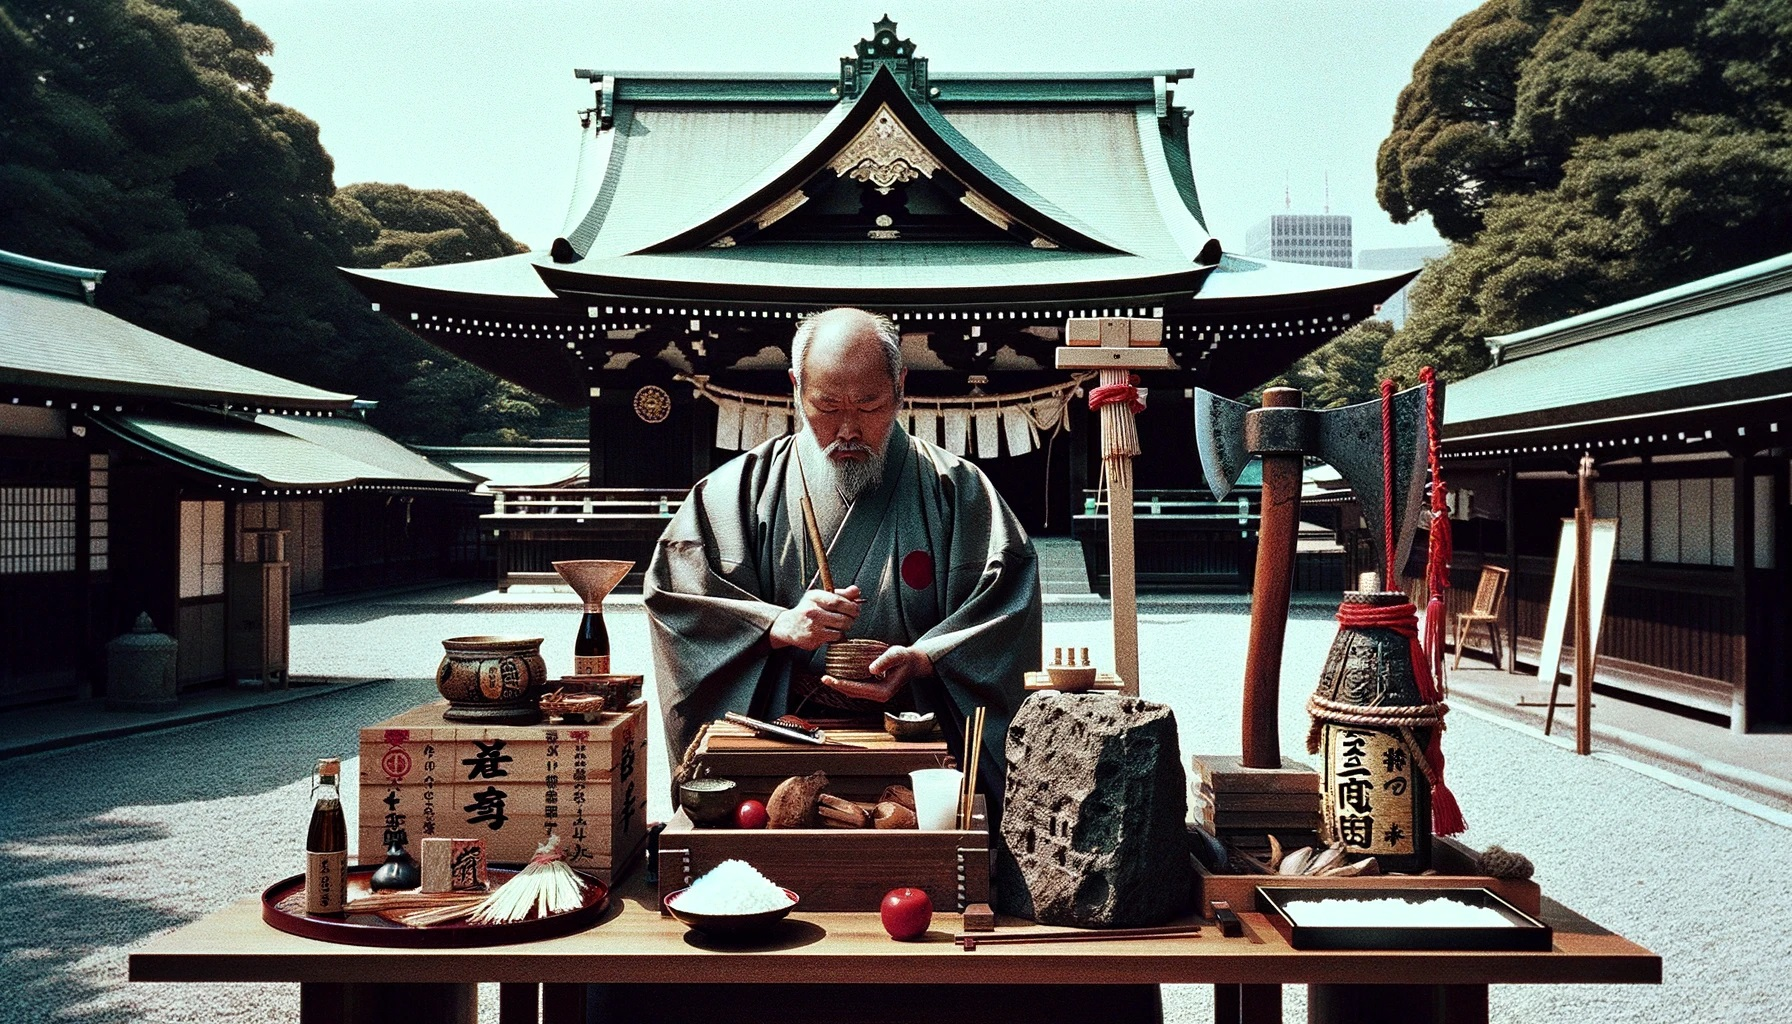
\includegraphics[width=0.8\textwidth]{shrine_offering.jpg}
    \caption{A Shinto priest performs a ritual offering at a shrine in Tokyo in the aftermath of the 2025 catastrophe. The offering includes traditional items such as rice, sake, and salt, as well as newer elements such as a hunter's weapon and a piece of dungeon debris, reflecting the adaptation of Shinto practices to the challenges of the post-catastrophe era.}
    \label{fig:offering}
\end{figure}

\end{document}
